\documentclass[12pt,a4paper]{report}
% package de langues 
\usepackage[french]{babel}
\usepackage[utf8]{inputenc}
\usepackage[T1]{fontenc}

% package pour référence de liens sur pdf 
\usepackage[pdftex]{hyperref} % liens
\usepackage{lastpage} % numéro de page
\usepackage{caption}

% package de formes de document 
\usepackage[left=2.5cm,
              right=2.5cm,
              top=2.5cm,
              bottom=2.5cm
             ]{geometry}
% pour les tableaux 
\usepackage{array,multirow,makecell} 
\newcolumntype{R}[1]{>{\raggedleft\arraybackslash }b{#1}}
\newcolumntype{L}[1]{>{\raggedright\arraybackslash }b{#1}}
\newcolumntype{C}[1]{>{\centering\arraybackslash }b{#1}}

% package pour la page de couverture 
\usepackage{graphicx}
\usepackage[cyr]{aeguill}
\usepackage{fancyheadings}
\usepackage{amsmath}
\usepackage{amsfonts}
\usepackage{amssymb}
\usepackage{geometry}
\usepackage{eso-pic}
\usepackage{tikz}
\usetikzlibrary{calc}


% nouvelle commande pour la forme 
%\fancyhf[OFC]{\thepage / \pageref{LastPage}}
\rfoot{\thepage / \pageref{LastPage}}
%\setcounter{tocdepth}{3}

% pakages de couleurs du document
\usepackage{color}
\usepackage{xcolor}


% package pour la chimie
\usepackage[version=4]{mhchem}


% package pour la visualisation du code
\usepackage{listings}
\definecolor{darkWhite}{rgb}{0.94,0.94,0.94}
 
\lstset{
  aboveskip=3mm,
  belowskip=-2mm,
  backgroundcolor=\color{darkWhite},
  basicstyle=\footnotesize,
  breakatwhitespace=false,
  breaklines=true,
  captionpos=b,
  commentstyle=\color{red},
  deletekeywords={...},
  escapeinside={\%*}{*)},
  extendedchars=true,
  framexleftmargin=16pt,
  framextopmargin=3pt,
  framexbottommargin=6pt,
  frame=tb,
  keepspaces=true,
  keywordstyle=\color{blue},
  language=python,
  literate=
  {²}{{\textsuperscript{2}}}1
  {⁴}{{\textsuperscript{4}}}1
  {⁶}{{\textsuperscript{6}}}1
  {⁸}{{\textsuperscript{8}}}1
  {€}{{\euro{}}}1
  {é}{{\'e}}1
  {è}{{\`{e}}}1
  {ê}{{\^{e}}}1
  {ë}{{\¨{e}}}1
  {É}{{\'{E}}}1
  {Ê}{{\^{E}}}1
  {û}{{\^{u}}}1
  {ù}{{\`{u}}}1
  {â}{{\^{a}}}1
  {à}{{\`{a}}}1
  {á}{{\'{a}}}1
  {ã}{{\~{a}}}1
  {Á}{{\'{A}}}1
  {Â}{{\^{A}}}1
  {Ã}{{\~{A}}}1
  {ç}{{\c{c}}}1
  {Ç}{{\c{C}}}1
  {õ}{{\~{o}}}1
  {ó}{{\'{o}}}1
  {ô}{{\^{o}}}1
  {Õ}{{\~{O}}}1
  {Ó}{{\'{O}}}1
  {Ô}{{\^{O}}}1
  {î}{{\^{i}}}1
  {Î}{{\^{I}}}1
  {í}{{\'{i}}}1
  {Í}{{\~{Í}}}1,
  morekeywords={*,...},
  numbers=left,
  numbersep=10pt,
  numberstyle=\tiny\color{black},
  rulecolor=\color{black},
  showspaces=false,
  showstringspaces=false,
  showtabs=false,
  stepnumber=1,
  stringstyle=\color{gray},
  tabsize=4,
  title=\lstname,
}

%package pour les algorithmes
\usepackage{algorithm}
\usepackage{algorithmic}
\usepackage{amsmath}

% package pour les tableaux
\usepackage{longtable}
\usepackage{booktabs}

% package pour les figures 
\usepackage{subcaption}

% package de reférencement
% \usepackage[backend=biber,safeinputenc, sorting=none]{biblatex}

% mettre la bibliographie dans la table de matières
%\usepackage[nottoc, notlof, notlot]{tocbibind}
\include{page_couverture.tex}


\author{MBE MBE MINDJANA LOIC HENRI}
\title{GNPS et MDByTE}

\begin{document}
    
    \pagecouverture
    {Plongement de graphes : GRAPH ATTENTION NETWORKS (GAT)}
    {}
    \tableofcontents
    \vspace{20cm}
    
    \section{Introduction}
    L'utilisation des méthodes de spectrométrie à savoir la spectrométrie de masse à haute résolution et par résonnance magnétique nucleaire pour la construction de réseau d'interprétation nommé \textbf{réseau moléculaire} par la suite, est très commun de nos jours, du moins sont très répendu du fait de la qualité des réseaux, des informations qu'ils contienent. Toute fois seul des sous graphes de ces réseaux nommés des clusters sont ciblées pour l'analyse, et dans l'article [Bioactivity-Based Molecular Networking for the Discovery of Drug Leads in Natural Product Bioassay-Guided Fractionation] où on a détecté une nouvelle molécule disposé entre deux clusters. Alors comment peut-on obtenir un graphe permettant de porter encore mieux les informations localement du réseau? On pourrait utiliser un réseau qui permettrait d'avoir un plongement du graphe tel que les réseaux de neuronnes GAT, Qu'est ce qu'un réseau de neuronne GAT et quelles sont ces caractéristiques ? 

    Dans les lignes qui suivent nous présenterons les réseaux GAT sur la base de son article de référence.

    \section{Contexte}
    Les réseaux de neurones convolutifs (CNN) ont été appliqués avec succès pour résoudre des problèmes tels que comme la classification d'images, la segmentation sémantique ou la translation (Gehring et al., 2016), où la représentation sous-jacente des données a une structure en forme de grille. Ces architectures réutilisent efficacement leurs filtres locaux, avec des paramètres apprenables, en les appliquant à toutes les positions d'entrée.Mais dans la réalité , tous les données ne sont pas représentées sous forme de tableau mais de graphes. 
    
    Des réseaux de neurones dit de graphe \textbf{GNN} ont été développés pour traiter les graphs directement en essayant de réaliser des plongements du graphe dans des espaces de graphe qui représenterais mieux le graphe d'entrée, on peut parler des GCN qui eux essayent de réealiser de la convolution de graphe toujours dans cette optique. Ils, c'est a dire les GCN et GNN ont cela en commun qu'ils ne pretent pas attention pour un noeud précis les informations contenus par ces voisins. D'ou la naissance des réseaux de neuronnes d'attentions.

   \section{Architecture d'un réseau GAT}
    Lorsqu'on parle d'une archiitecture d'un réseau de neuronnes, on se refère généralement à la succession de couches de ce réseau en définissant leurs types caractérisés par les opérations qu'elles éffectuent. Nous parlerons dont ainsi de la couche caractérisant les réseaux GAT et ainsi du moyens des mis a jour des parametres globalement de ces couches.  

    \subsection{Couche attentionelle (GRAPH ATTENTIONAL LAYER)}
    Les premièrs éléments à identifier pour une couche de neuronnes est l'entrée et la sortie de la couche. A l'entree on a un graphe et en sortie également un graphe englobant plus généralement les informations du graphe d'entrée par son processus. 

    On a ainsi un ensemble de \emph{N} noeuds, $h =\{ \overrightarrow{h_{1}},\overrightarrow{h_{2}}...,\overrightarrow{h_{n}} \}$ où $h_{i}$ représente le noeud i de $F$ caractéristique(s) réelle(s); et en sortie on a un ensemble de \emph{N} noeuds $h' =\{ \overrightarrow{h'_{1}},\overrightarrow{h'_{2}}...,\overrightarrow{h'_{n}} \}$ où $h'_{i}$ représente le noeud i de $F'$ caractéristique(s) réelle(s).

    Pour calculer le coefficient d'attention entre un noued $h_{i}$ et $h_{j}$, on utilise la fonction 
    $$ e_{ij} = a'(Wh_{i}, Wh_{i}) $$
    \begin{center} où \end{center}
    $$a'(Wh_{i}, Wh_{i}) = a^{T}[Wh_{i}||Wh_{i}]$$ avec $
    a (2 F')$ étant le vecteur d'attention à apprendre du graphe, et $W( F' \times F)$ la matrice de poids tel un noyau de convolution à apprendre.

    Afin de rendre les coefficients comparables par voisinage on normalise l'ensemble des coefficients, et on obtient le coefficient 
    $$ \alpha_{ij} = \frac{ \exp(LeakyReLU(e_{ij})) }{\sum_{k\in \eta_{j}}^n \exp(LeakyReLU(e_{ik})) } $$

    Ayant les coefficient $\alpha_{ij}$, on cherche à obtenir sur la base d'un noeud i et son voisinage $\eta_i$, un noeud j qui sera une intégration de ce noeud dans une nouvelle dimension.

    \begin{center}
        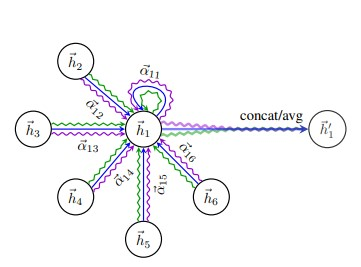
\includegraphics{Images/GAT1.jpg}
        
         \emph{Figure: Accumulation d'informations du voisinage d'un noeud et du noeud}
    \end{center}
    
    En utilisant une fonction d'agrégation $ \sigma $ telque la moyenne, on peut comprendre, la formule vectorielle de l'opération de calcul du noeud  $h'_{i}$ issu de $h_{i}$ et de son voisinage $\eta_{i}$ comme suit:
    $$
    h'_{i} = \sigma( \sum_{ i \in \eta_{i} } \alpha_{ij}(Wh_{i}) )
    $$

    \subsection{Couche attentionelle Multitete (GRAPH MULTIHEAD ATTENTIONAL LAYER)}
    Cette couche est semblable à la couche précédente mais possede $K$ attentions
    avec chacune ayant une matrice de projection. Ainsi on pourrai soit conserver les informations issues des attentions par concaténation de données
    $$
    h'_{i} = {\overset{K}{\underset{k=1}{||}} \sigma( \sum_{ i \in \eta_{i} } \alpha^{k}_{ij}(W^{k}h_{i}) )  }
    $$ 
    ou soit les accummuler ces informations par agglomération ou encore aggrégation
     $$
    h'_{i} =  \sigma( \frac{1}{K} \sum_{ k = 1 }^K \sum_{ i \in \eta_{i} } \alpha^{k}_{ij}(W^{k}h_{i}) ) )
    $$

    Afin de mettre à jour les poids des paramètres d'attentions et matrice de poids par rapport au deux couche on utilise l'algoithme de rétroprogation de l'érreur qui s'appui sur le fait, qu'on devrait mettre à jour les valeurs des paramètres sur des erreurs des sorties et des erreurs obtenus sur l'operation  par rapport à eux memes. Il faut aussi noter que les érreurs des éntrées par rapport à l'opération doivent etre aussi calculer afin d'etre propager à la couche précédente. 
    
    On parle alors là de calcul différentielle de la fonction d'opération par rapport auux entrées et aux sorties, vues que par rapport à la sortie est obtenues soit de la couche suivante, soit la fonction d'érreur d'évaluation.
    
    \section{Conclusion}
    Il étatt question pour nous de présenter les réseaux de 'neuronnes' de graphe d'attention GAT, de manière plus précise s'il pouvait bien évidemment ètre utiliser pour réealiser une agglomération de connaissance issues de réseaux moléculaires qu'on peut obtenir des techniques de spectrométrie HRMS et RMN dans le but de les amméliorer. La question à ce poser à ce niveau est celle de savoir si d'un point de vue thématique de telles opérations sont pertinentes? Et aussi qu'elles sont véritablement les formules associés à la rétropropagations de l'érreur pour des couche de ce type de réseaux ?Mais A ce niveau nous pensons pouvoir le faire dans les jours qui suivent.

    
  \bibliographystyle{unsrt}
    \bibliography{reference_GNPS_MADByTE}
\end{document}